\documentclass[letterpaper]{article}
\usepackage{alltt}
\usepackage{graphicx}
\usepackage{xspace}
\usepackage{color}
\definecolor{linkcolor}{RGB}{16,65,69}

\newcommand{\ttt}[1]{\texttt{#1}}
\newcommand{\projname}{\ttt{bt}\xspace}

\newenvironment{monospace}{\begin{quote}\begin{alltt}}{\end{alltt}\end{quote}}

\author{Joe Colosimo \\ \small{colosimo@mit.edu} \\ Group 6}
\date{\today}

\usepackage[colorlinks=true, linkcolor=linkcolor]{hyperref}
\title{\projname{} - A Realtime Beat Tracker \\ First Test Results}
\begin{document}

\maketitle

\section{Status}

The overall system is working.  As described in the original architecture
design, the beat classifier injects beat events into all of the metronomes,
which currently just reset their counters to 0.  The metronomes are just
counting a 4-4 beat, so subdivision is not implemented yet.  With each beat
event, all of the metronome phase errors are collected and then fed out via an
output FIFO, which interfaces with the top level serial module.

The serial output goes into a command-line (don't laugh) program that spits out
some ASCII art, as shown in Figure~\ref{fig:swscreenshot}.  In this example,
I'm feeding in a 126-BPM track with a very strong beat

    \begin{figure}
        \centering
        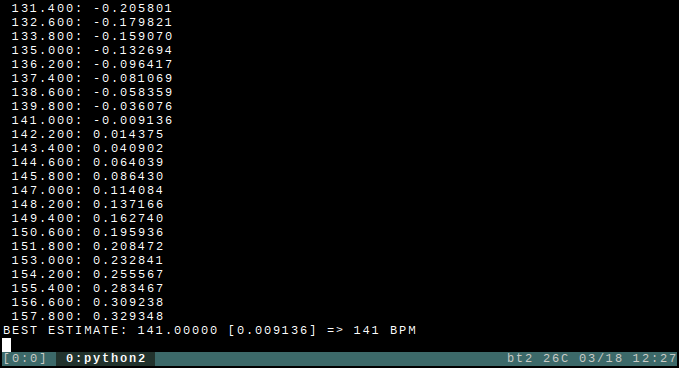
\includegraphics[scale=.3]{fig/swscreenshot.png}
        \caption{Serial output from the FPGA is received by the software and
            displayed by this amazing software script.}
        \label{fig:swscreenshot}
    \end{figure}

However, it doesn't do so well for everything.  The main issue is that the beat
classifier isn't quite right yet.  But on top of that, inaccuracies in the beat
classifier can be smoothed by messing with some of the phase correction
settings.  For example, instead of correcting the phase to 0, it would be
better to correct the phase to something like halfway between 0 and the current
phase offset.  This will help prevent incorrect classifications from causing
too much damage.


\section{Next Steps}

Based on my observations, I think that it's not going to be useful to implement
field narrowing.  So, I'm going to redesign the metronome modules to be
instantiated with a singular tempo.  I'm currently able to meet timing even
fitting upwards of 120 metronomes on the chip.

Secondly, I'm going to do some preliminary tuning with the phase error
correction feature of the metronomes, as discussed above.

Third, I'm going to try to improve the beat classification as much as possible.
I'd like to still use an energy-based approach, but this time, I'm going to
look at the variance of the last $N$ energy samples and use that to build the
threshold for beat classification instead of just using a fixed constant of
1.25.  I think this will improve accuracy greatly, as I've seen
examples\footnote{\url{http://www.flipcode.com/misc/BeatDetectionAlgorithms.pdf}}
that illustrate the point that a variable threshold works significantly better
than a fixed threshold. 

\end{document}
